\section{Цель работы}
Цель настоящей работы --- освоить средства моделирования задач линейного программирования.

\section{Задание}
\textit{Вариант 16.}
Кондитерская фабрика для производства трёх видов карамели А, В и С использует три вида основного сырья: сахарный песок, патоку и фруктовое пюре. Нормы расхода сырья каждого вида на производство 1 т карамели данного вида приведены в таблице.
В ней же указано общее количество сырья каждого вида, которой может быть использовано фабрикой, а также приведена прибыль от реализации 1 т карамели данного вида.

\begin{table}[H]
\begin{tabular}{llllll}
Вид сырья      & A   & B   & C   & Объем ресурса & \\
\hline
Сахарный песок & 0.8 & 0.5 & 0.6 & 800 & \\
Патока         & 0.4 & 0.4 & 0.3 & 600 & \\
Фруктовое пюре & -   & 0.1 & 0.1 & 120 & \\
\hline
Прибыль от реализации 1 т продукции (р.) & 108 & 112 & 126 &
\end{tabular}
\end{table}

Найти план производства карамели, обеспечивающий максимальную прибыль от её реализации.

\section{Поставленная задача}
\begin{gather*}
108x_1 + 112x_2 + 126x_3 \rightarrow max \\
0.8x_1 + 0.5x_2 + 0.6x_3 \le 800 \\
0.4x_1 + 0.4x_2 + 0.3x_3 \le 600 \\
0.1x_2 + 0.1x_3 \le 120 \\
x_1, x_2, x_3 \ge 0
\end{gather*}

\newpage

\section{Решение в Excel}
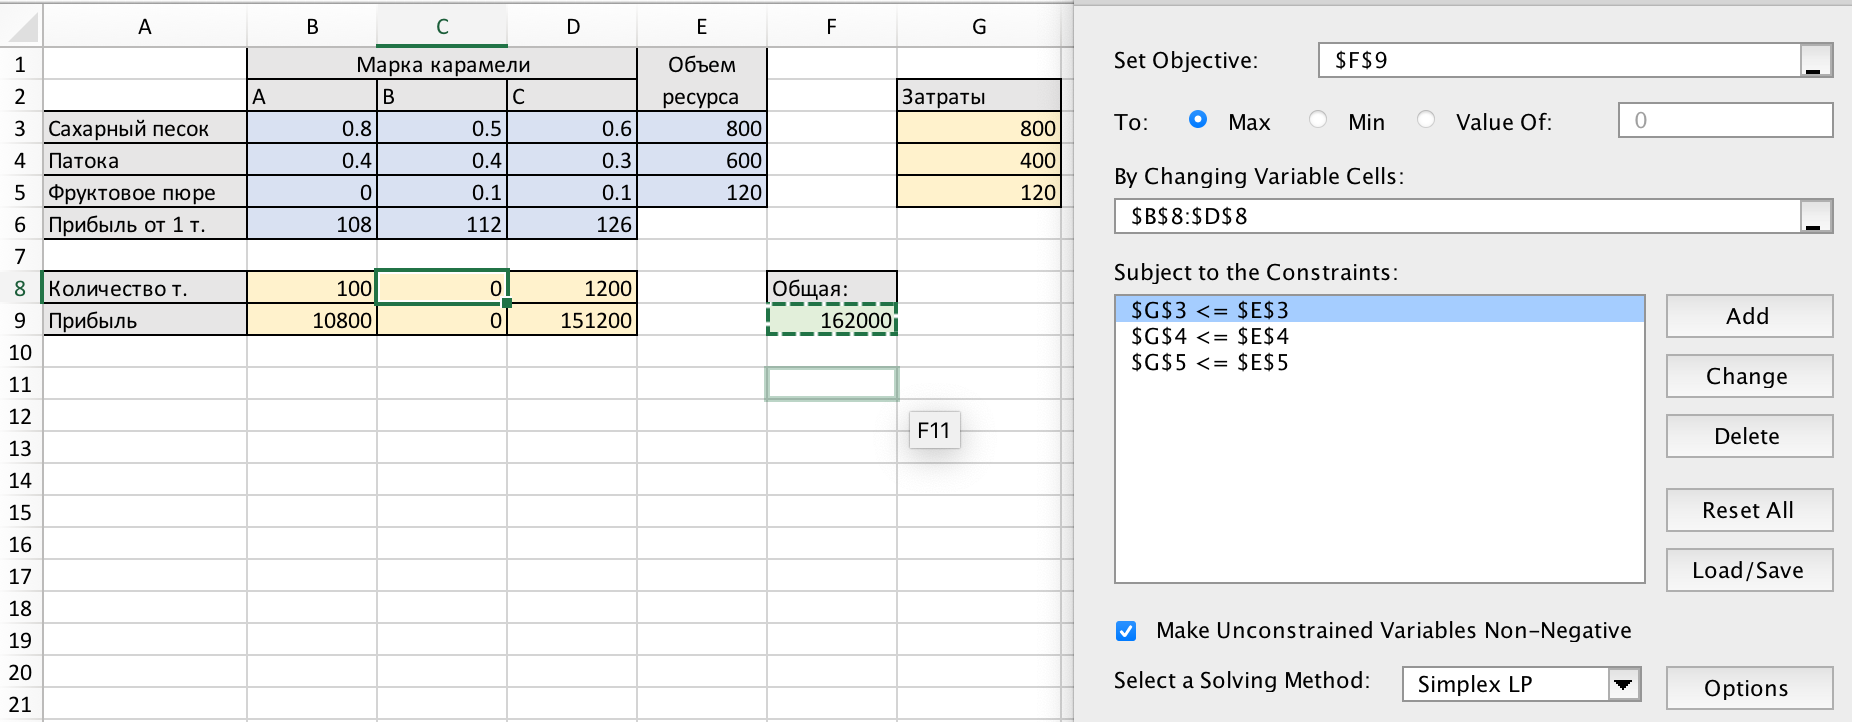
\includegraphics[width=\textwidth]{excel}

\section{Решение с использованием Python}
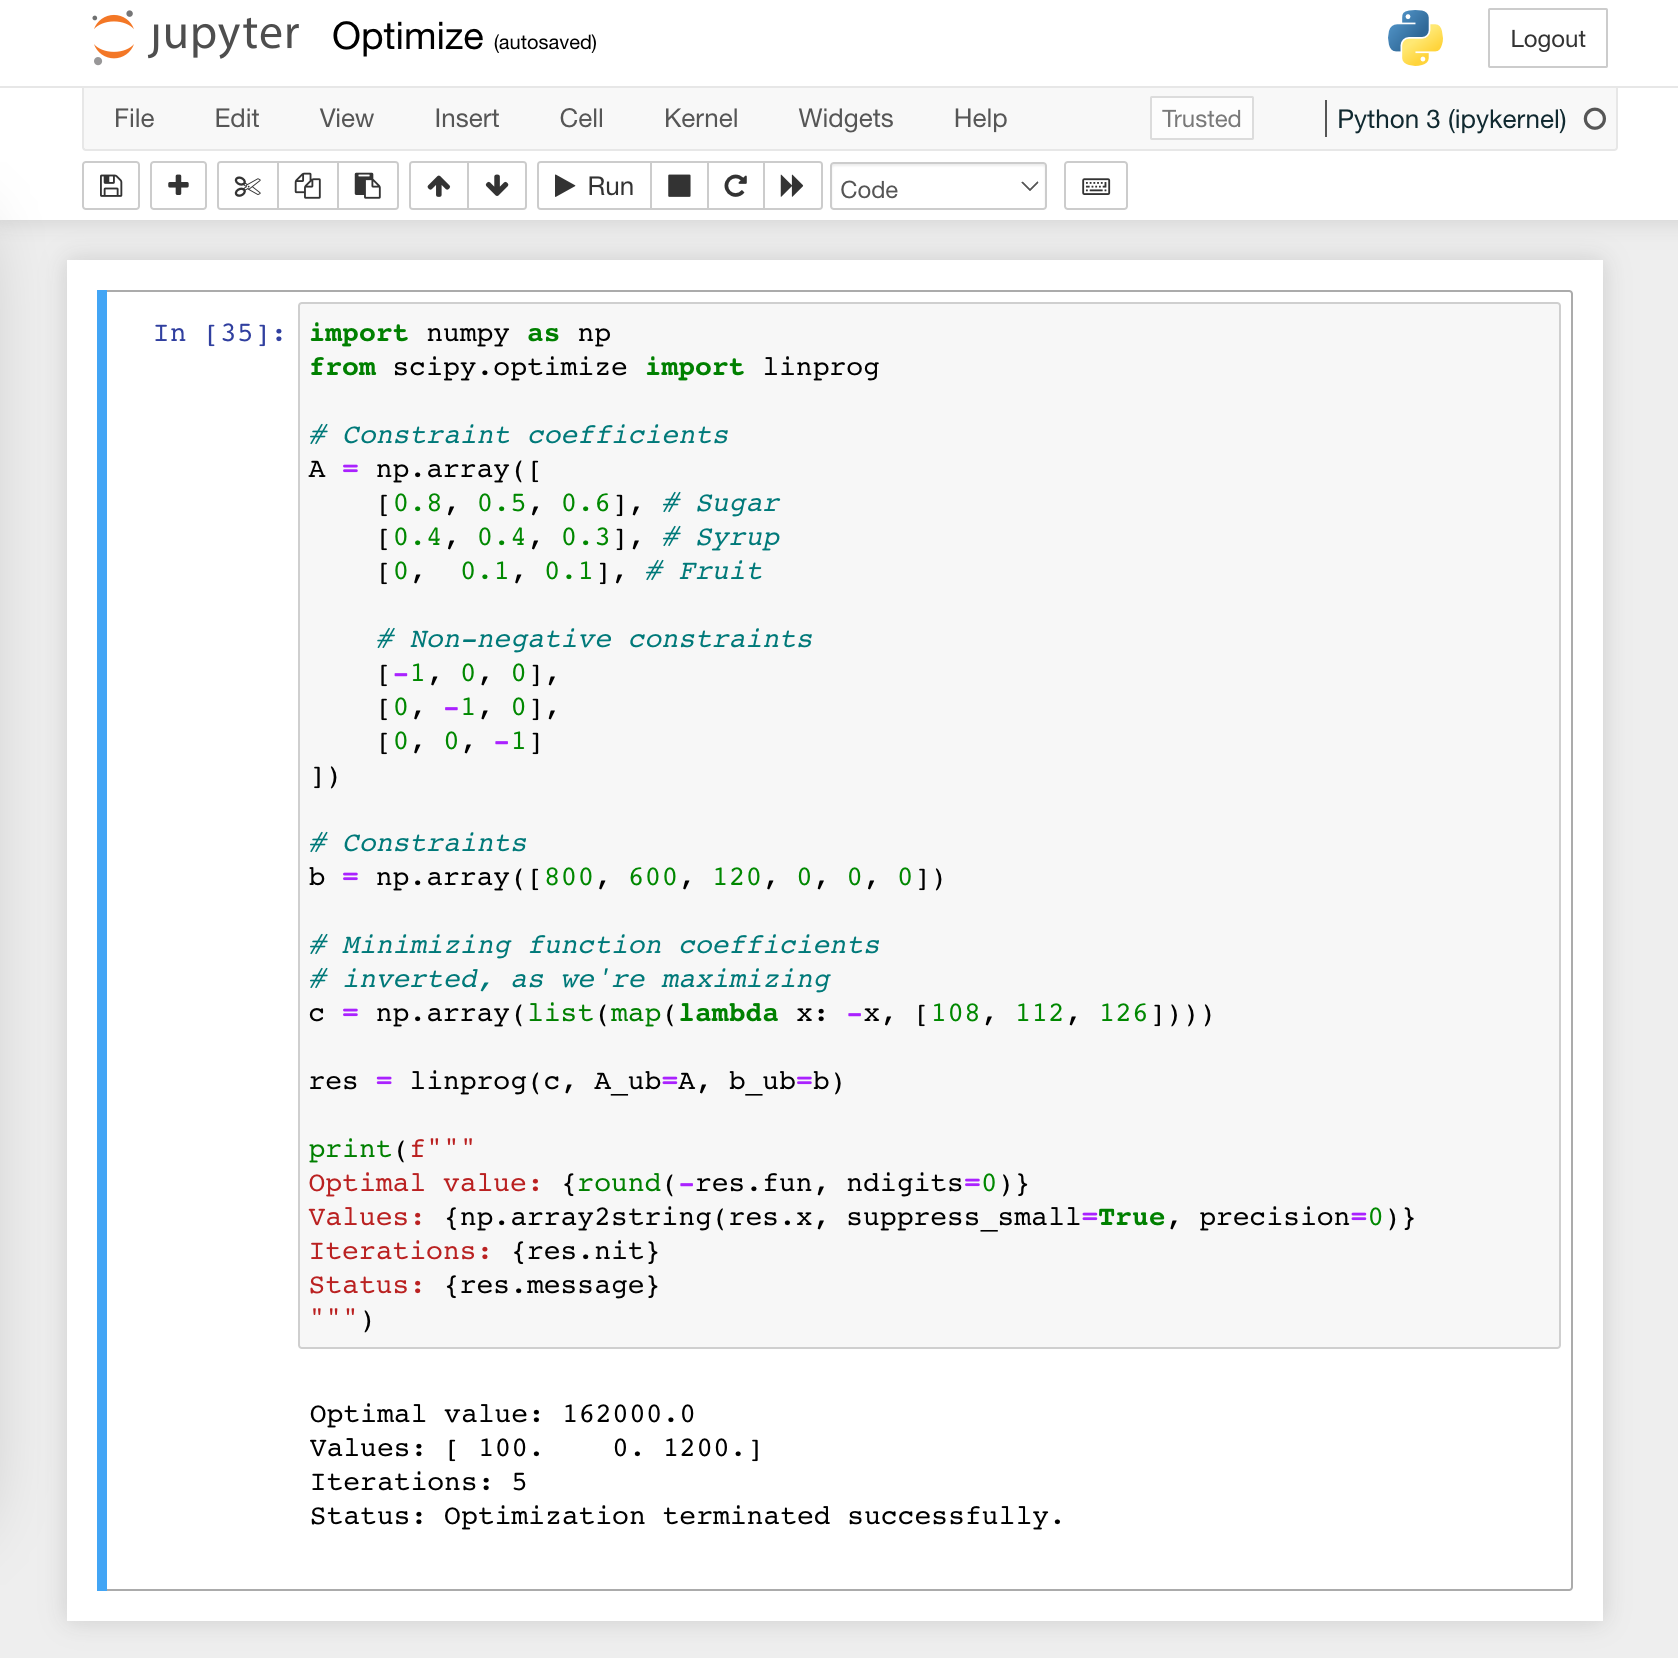
\includegraphics[width=0.9\textwidth]{jupyter}

\newpage

\begin{verbatim}
Optimal value: 162000.0
Values: [ 100.    0. 1200.]
Iterations: 5
Status: Optimization terminated successfully.
\end{verbatim}

\section{Приложение 1. Код программы на Python}
\begin{minted}{python}
import numpy as np
from scipy.optimize import linprog

# Constraint coefficients
A = np.array([
    [0.8, 0.5, 0.6], # Sugar
    [0.4, 0.4, 0.3], # Syrup
    [0,  0.1, 0.1], # Fruit

    # Non-negative constraints
    [-1, 0, 0],
    [0, -1, 0],
    [0, 0, -1]
])

# Constraints
b = np.array([800, 600, 120, 0, 0, 0])

# Minimizing function coefficients
# inverted, as we're maximizing
c = np.array(list(map(lambda x: -x, [108, 112, 126])))

res = linprog(c, A_ub=A, b_ub=b)

print(f"""
Optimal value: {round(-res.fun, ndigits=0)}
Values: {np.array2string(res.x, suppress_small=True, precision=0)}
Iterations: {res.nit}
Status: {res.message}
""")
\end{minted}
